\section{Ex2.11 Reading data}\label{sec:Reading_data}

\subsection{Testo esercizio}
Il file \verb|trajectory.dat| contiene un elenco di numeri:\\   
\begin{tabular}{ccc}
    $t0$    & $x0$      & $y0$    \\
    $t1$    & $x1$      & $y1$    \\
    $\dots$ & $\dots$   & $\dots$ \\
    $tn$    & $xn$      & $yn$    \\
\end{tabular}\\
corrispondente al tempo $t(i)$ misurato in secondi e alle posizioni $x(i)$ e 
$y(i)$  misurato in metri per la traiettoria di un proiettile.
    
\begin{itemize}
    \item[a)] Leggere il file di dati, e popolare le matrici $t$, $x$ e $y$.
        
    \item[b)] Tracciare le posizioni $x$ e $y$ in funzione del tempo in due 
    grafici uno sopra l'altro.
        
    \item[c)] Tracciare le posizioni $(x, y)$ dell'oggetto in un grafico 
    con $x$ e $y$ sui due assi.
\end{itemize}

\subsection{Svolgimento}
Per questo esercizio ho deciso di usare le funzioni integrate dell'IDE di 
MATLAB che offrono una gestione dei file molto più comoda rispetto a quella con 
\verb*|fopen()|. Infatti con un file correttamente formato, basta una sola 
istruzione per importare i dati da un file. Poi con tre semplicissime 
assegnazioni, ottengo le tre variabili richieste. In seguito, ho deciso di 
mostrare tutti i 3 grafici insieme per rendere visibile in un'unica finestra 
tutti i risultati.
\subsection{Grafico}
\begin{figure}[h]
    \centering
    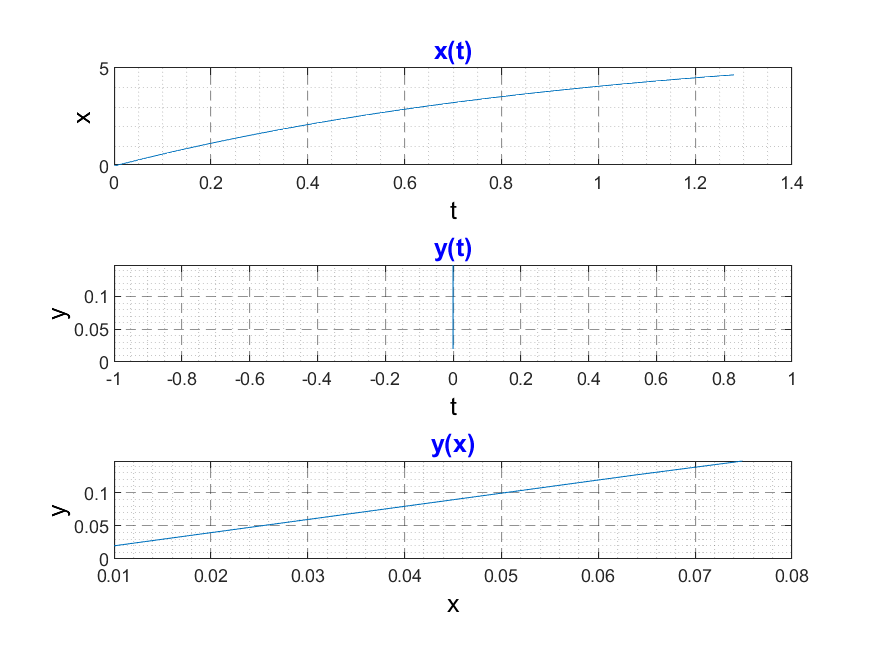
\includegraphics{cap/Elementary/img/script211}
    \label{fig:script211}
\end{figure}

\subsection{Codice esercizio}
\lstinputlisting[title = {\nameref{sec:script211}},
linerange={3-25}]
{cap/Elementary/src/script/script211.m}